\section{Experimentos numéricos}

\subsection{OCP for SHE with symmetry of quarter-cycle}
To solve the optimal control problem (\ref{OCP_bn}), we use a direct method. 
If we consider a partition $\mathcal{P} = \{\tau_0,\tau_1,\dots,\tau_{T}\}$ of interval $[0,\pi/2]$ , we can represent a function $\{ f(\tau) \ | \ \tau \in [0,\pi/2]\}$ as a vector $\bm{f} \in \mathbb{R}^{T}$ where component $f_t = f(\tau_t)$. Then the optimal control problem (\ref{OCP_bn}) can be written as optimization problem with variable $\bm{f} \in \mathbb{R}^{T}$. In this way we solve the next problem:

\begin{problem}
    Given  a set of odd numbers $\mathcal{E}_b$ with carinality $|\mathcal{E}_b| = N_b$, given the target vector $\bm{b}_T  \in \mathbb{R}^{N_b}$ and  partition $\mathcal{P} = \{\tau_0,\tau_1,\dots,\tau_{T}\}$ of interval $[0,\pi/2]$. We search a vector $\bm{f} \in \mathbb{R}^{T}$ that minimize the following function:
    \begin{gather}
        \min_{\bm{f} \in \mathbb{R}^{T} } \Bigg[ || \bm{b}_T - \bm{\beta}^{T}||^2 - \epsilon  \sum_{t=0}^{T} f_{t}^2 \Delta\tau_t  \Bigg]  \\
        \notag \text{suject to: } \\
        \notag j \in \mathcal{E}_b \ \ 
        \begin{cases}
            \beta_j^{t+1} = \beta_j^{t} + \Delta \tau_t (4/\pi) \sin(j\tau_t) f_t \\
            \beta_j^0 = 0
        \end{cases} \\
        \notag |f_t| < 1 \ | \ \forall t \in \{1,\dots,T\} \\
        \Delta \tau_t = \tau_{t+1} - \tau_{t} \ | \ \forall t \in \{2,\dots,T\}
    \end{gather}
\end{problem}

This problem is a nonlinear programming, for this we use CasADi software to solve.

\subsubsection{Numerical result for SHE of two levels}

We considered the set of odd numbers $\mathcal{E}_b = \{1,5,7,11,13\}$ and a target vector $\bm{b}_T = [m_a,0,0,0,0]$, where $m_a \in [0,1]$ is a parameter . We will compare the three solutions of problem (\ref{SHEp_clas}) (obtained via genetic algorithms) with a solutions of the optimal control problem (\ref{OCP_bn}) with three penalization terms: $\mathcal{L}[f] = -f$, $\mathcal{L}[f] = +f$ and $\mathcal{L}[f] = -f^2$ obtained by direct method with uniform partition of interval $[0,\pi/2]$ with $T=400$ and penalization parameter $\epsilon = 10^{-5}$. To obtain the solutions of problem (\ref{SHEp_clas}) we considered the number of switching angles $M=5$. 

Mostramos en la figura (\ref{fig:error_solutions}) los errores para tres soluciones obtenidas mediante algoritmos genéticos del problema (\ref{SHEp_clas}) y tres soluciones obtenidas mediante control óptimo con los distintos términos de penalización.  Esto nos asegura que el orden de magnitud de las soluciones obtenidas son del mismo orden. Además podemos ver en la figura (\ref{fig:solutions}) que el control óptimo con los términos $\mathcal{L}[f] = -f$ y $\mathcal{L}[f] = +f$ recuperar dos soluciones obtenido del problema (\ref{SHEp_clas}). Mientras que el problema de control con el término $\mathcal{L}[f] = f^2$ es solución del problema pero no presenta continuidad con respecto $m_a$.
 
\begin{figure}[!ht] 
        \centering
        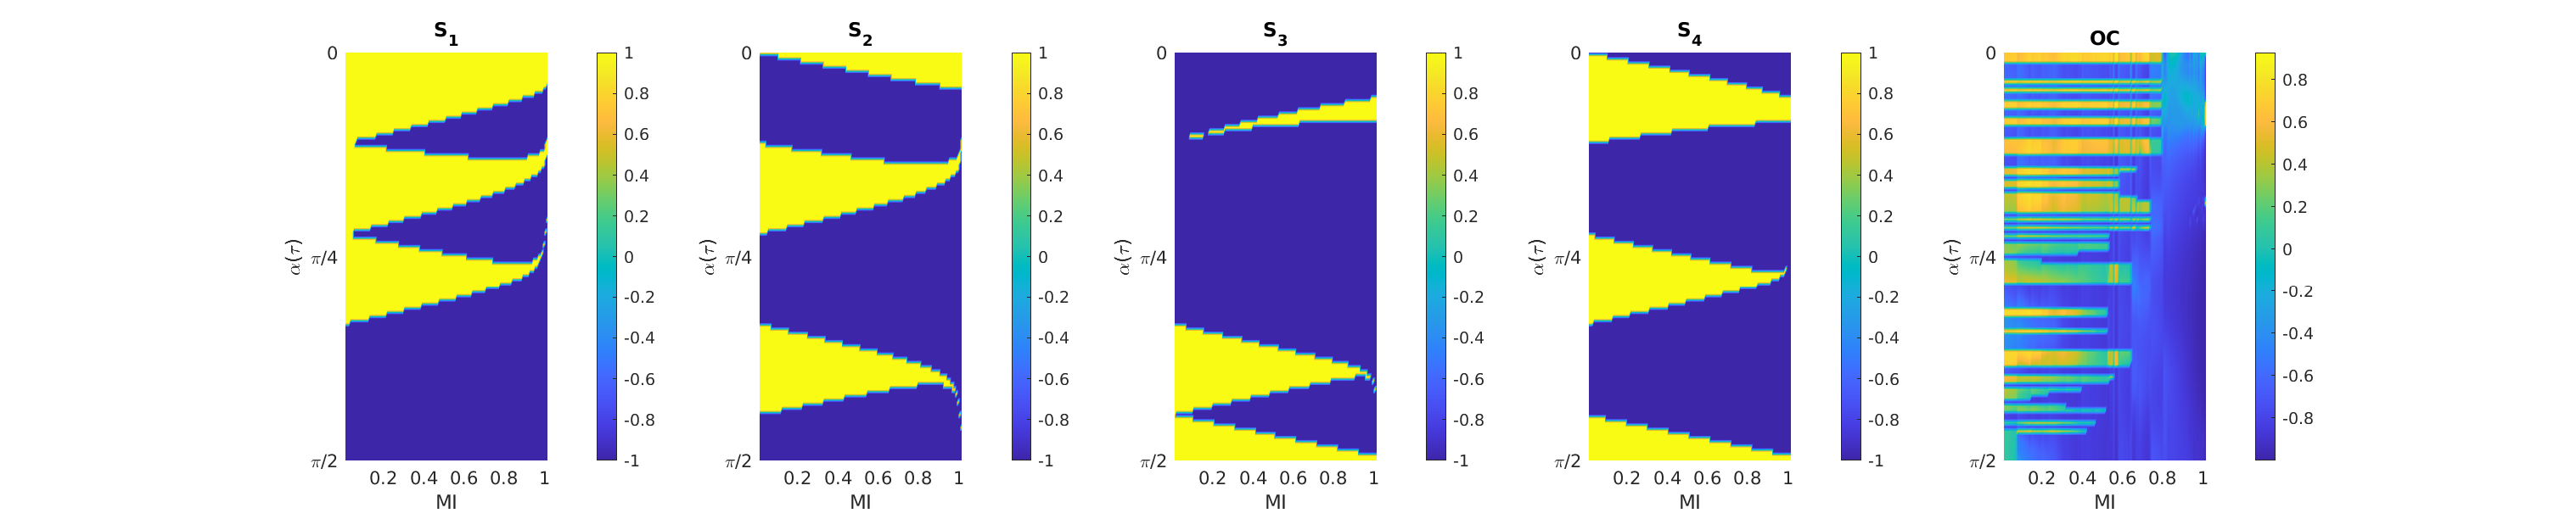
\includegraphics[scale=0.5]{img/EX01_surf.eps}
        \caption{Comparison of solutions for different values of $m_a$. Solutions $S_1$, $S_2$, $S_3$ correspond to problem (\ref{SHEp_clas}) where the number of switching angles is prefixed, while $OC$ solution correspond to optimal control problem.}
        \label{fig:solutions}
    \end{figure}


 
\begin{figure}
    \centering
    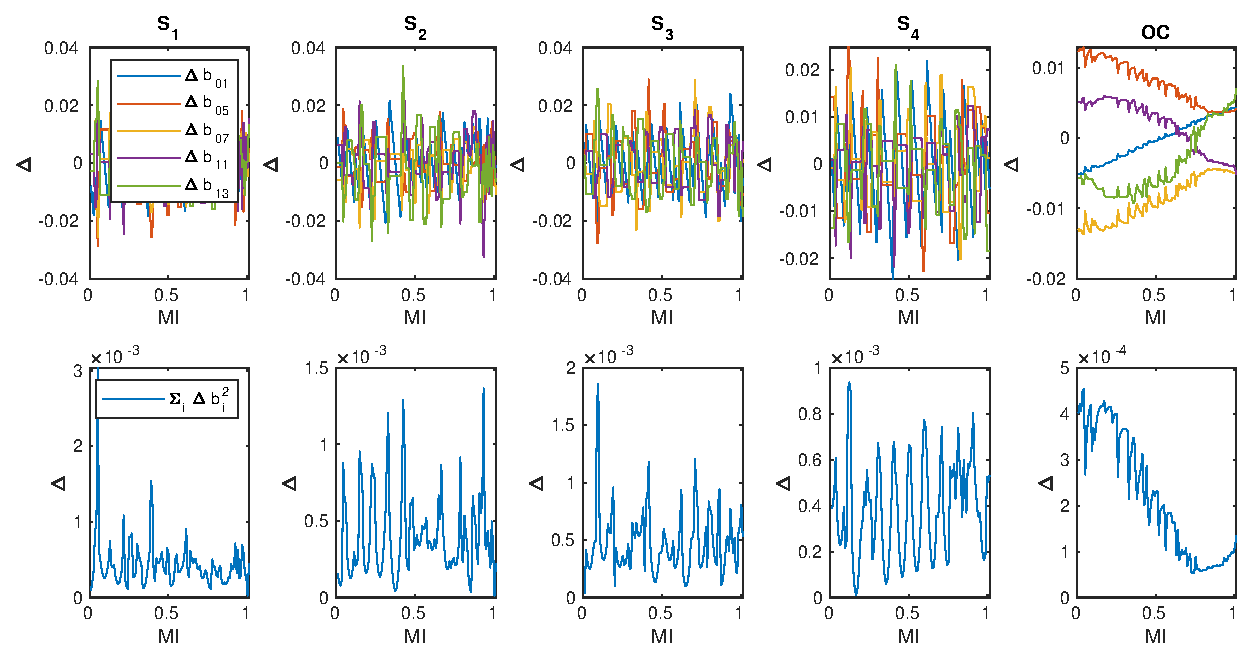
\includegraphics[scale=0.5]{img/EX01.eps}
    \caption{The order of magnitud of the square of euclidean distantes to target is the same for all solutions of figure (\ref{fig:solutions})}
    \label{fig:error_solutions}
\end{figure}

\subsubsection{Numerical result for SHE of three levels}

Podemos ver que en el caso en el que el control $f(\tau)$ solo pueda tomar valores entre $[0,1]$ obtenemos señales que pueden tomar tres niveles en el intervalo $[0,2\pi]$ gracias a la simetría de cuarto de onda. Si resolvemos el problema de control óptimo pero esta vez cambiando las restricciones $|f(\tau)|<1$ por $\{0<f(\tau)<1\}$. Se ha realizado el mismo procedimiento que en el caso anterior, obteniendo soluciones para los mismo términos de penalización.

\begin{figure}
    \centering
    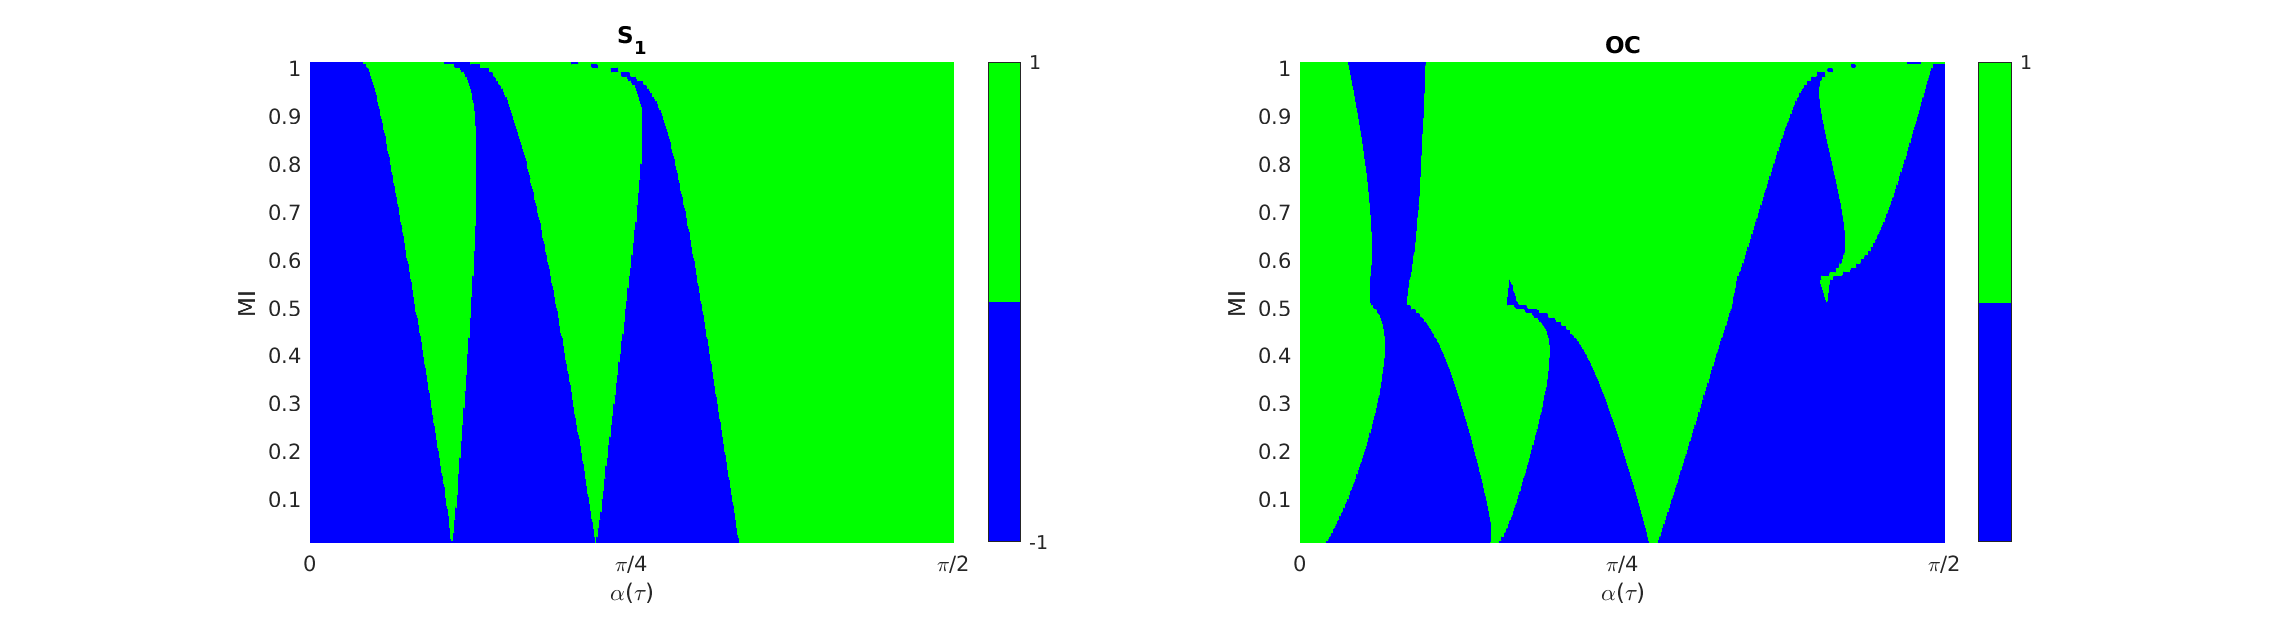
\includegraphics[scale=0.45]{img/EX01_surf_3LVL.eps}
    \caption{Soluciones para un control  con restriciones $0 \leq f\leq 1$ para obtener soluciones de tres niveles.}
\end{figure}

\begin{figure}
    \centering
    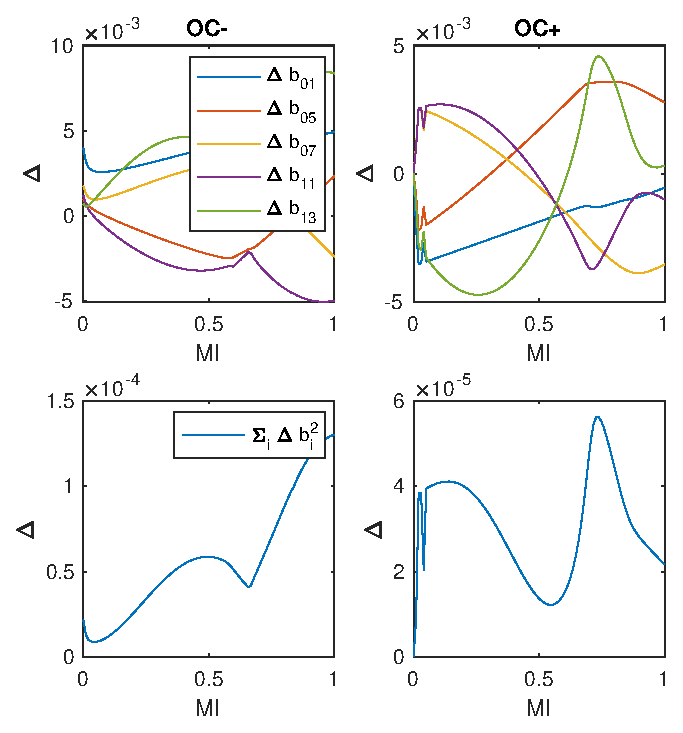
\includegraphics[scale=0.7]{img/EX01_3LVL.eps}
    \caption{Errors of solution in three level solutions}
\end{figure}


\subsection{OC for SHE with symmetry of half-cycle}